% Point to the main file
\documentclass[../../Main.tex]{subfiles}

% ========== Start the document ==========
\begin{document}

\section{Section 4.3 - Primes}

\begin{definition}
    A \yellowbox{prime number} is a positive integer with exactly \textbf{2 distinct factors}
\end{definition}

\begin{example}
    Here are the first few primes

    $2, 3, 5, 7, 11, 13, 17, 19, 23, 29, 31, 37, \ldots$

    is 257 prime?
    
    We use \textbf{trial division}

    We'll use a loop

    \begin{lstlisting}[language=Python]
        for k = 2 to 256
            if 257 % k = 0
                then return "composite"
            else
                k += 1
    \end{lstlisting}

    For efficiency, we could just go up to $\sqrt{257}$, or $\lfloor \sqrt{256} \rfloor$

    Second method: \textbf{Sieve of Eratostheres}

    \begin{tabular}{c c c c c c c c c c}
        1 & 2 & 3 & 4 & 5 & 6 & 7 & 8 & 9 & 10 \\
        11 & 12 & 13 & 14 & 15 & 16 & 17 & 18 & 19 & 20 \\
        21 & 22 & 23 & 24 & 25 & 26 & 27 & 28 & 29 & 30 \\
        31 & 32 & 33 & 34 & 35 & 36 & 37 & 38 & 39 & 40 \\
        41 & 42 & 43 & 44 & 45 & 46 & 47 & 48 & 49 & 50 \\
    \end{tabular}

    I honestly forgot how this works since I didn't write it down too well

    Third method: \textbf{Fermat's Method}

    if $n = a^2 - b^2$

    then $n = (a - b)(a + b)$

    Check: $a - b > 1$ and $a + b > 1$

    If neither is 1, then $n$ is composite
    If both are greater than 1, then they can't be $n$

    Fourth Method: \textbf{Quadratic Sieve}

    Solve $$a^2 - b^2 \equiv 0 \pmod{n}$$

    Then $$n \mid a^2 - b^2 \implies a^2 - b^2 = nk, k \in \setZ$$

\end{example}

\begin{proposition}
    There are infinitely primes

    \begin{poof}
        Suppose on the contrary, there are finitely many primes such that all primes can be written like

        $$p_1, p_2, \ldots, p_k$$

        Consider $$N = p_1 p_2 \cdot \ldots \cdot p_k + 1$$

        Case 1: Suppose $N$ is prime

        That means that
        \begin{center}
            N is larger than $p_i$ for $i = 1, 2, \ldots, k$ \\
            Hence $N \not = p_i$ for $i = 1, 2, \ldots, k$
            We have a contradition of our finitely many primes!
        \end{center}

        Case 2: $N$ is composite

        Then $N$ must have a prime factor in the list $p_1, p_2, \ldots, p_k$

        Suppose $p_j$ is a prime factor of $N$

        Then $p_j \mid N$ and not $p_j \mid p_1 p_2 \cdot \ldots \cdot p_k$

        Then we conclude

        $$p_j \mid (N - p_1 p_2 \cdot \ldots \cdot p_k)$$

        Therefore

        $$p_j \mid 1, \; \text{is a contradition}$$

        We conclude there are infinitely primes, as desired (by contradition)
    \end{poof}
\end{proposition}

\begin{definition}[Prime Counting Function (Pi)]
    The function $\pi: \setR^+ \rightarrow \setZ^+$ is defined by

    \begin{align*}
        \pi(x) = \text{number of primes less than or equal to $x$}
    \end{align*}

    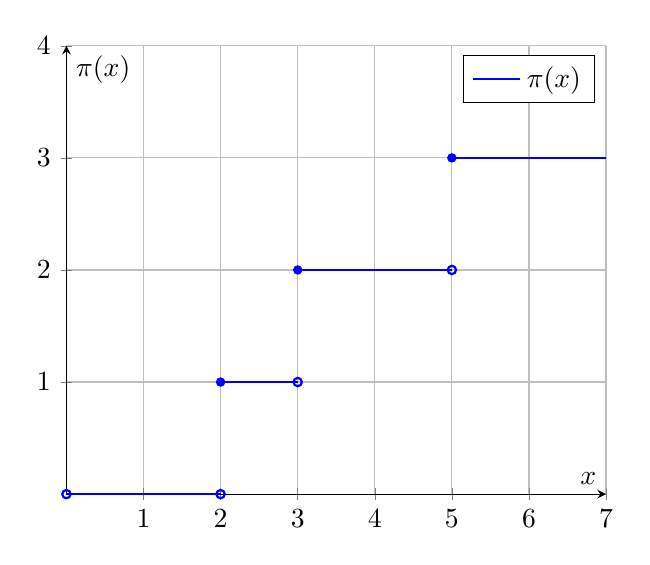
\begin{tikzpicture}
            \begin{axis}[
                unbounded coords=jump,
                axis lines=middle,
                xmin=0, xmax=7,
                ymin=0, ymax=4,
                xlabel=$x$, ylabel=$\pi(x)$,
                grid=both
            ]
                % Plotting a line
                % \addplot[
                %     blue, 
                %     thick, 
                %     domain=-3:3, 
                %     samples=7, % One sample per integer step
                %     jump mark left
                %     % const plot
                % ] {floor(x)};
                \addlegendentry{$\pi(x)$}

                \addplot[
                    const plot, 
                    blue, 
                    thick
                ] coordinates {
                (0, 0) (2, 0) (nan, nan) 
                (2, 1) ( 3, 1) (nan, nan)
                (3, 2) (5, 2) (nan, nan)
                (5, 3) (7, 3)
                % (0,0) (1,0) (2,1) (3,2) (4,2) (5,3) (6,3) (7,4) (8,4) (9,4) (10,4) 
                % (11,5) (12,5) (13,6) (14,6) (15,6) (16,6) (17,7) (18,7) (19,8) (20,8)
                };

                % 2. Add Closed Circles (Left end: Included)
                \addplot[
                    only marks, 
                    mark=*, 
                    mark size=1.5pt, 
                    blue
                ] coordinates {
                    (2, 1) (3, 2) (5, 3)
                };

                % 3. Add Open Circles (Right end: Excluded)
                \addplot[
                    only marks, 
                    mark=o, 
                    mark size=1.5pt, 
                    thick, 
                    blue, 
                    fill=white % This hides the grid/axis behind the circle
                ] coordinates {
                    (0, 0) (2, 0) (3, 1) (5, 2)
                };
                
                % Marking points
                % \addplot[only marks, mark=*, red] coordinates {(1,0) (3,2)};
                % 
                % \node[anchor=west] at (axis cs:3,2) {A(3,2)};
            \end{axis}
        \end{tikzpicture}

\end{definition}

\begin{theorem}[The Prime Number Theorem]
    
    This theorem is defined that $\pi(x)$ is approximately equal to $\frac{x}{\ln(x)}$ as $x \rightarrow \infty$

    $$\lim_{x \rightarrow \infty} \frac{\pi(x)}{\frac{x}{\ln(x)}} = 1$$

    In other words,

    $$\pi(x) \approx \frac{x}{\ln(x)}$$

    \begin{note}
        This was proven independenlty by Jacques Hadamard and Charles Jean de la Vallee Poussin in 1896
    \end{note}
\end{theorem}

To recap, we know so far for $a, b, c, d \in \setZ, m \in \setZ^+$ that

\begin{enumerate}
    \item $a \equiv b \pmod{m} \iff m \mid (a-b)$
    \item
    {
        $a \equiv b \pmod{m}, c \equiv d \pmod{m}$

        \begin{romanlist}
            \item $a + c \equiv b + d \pmod{m}$
            \item $ac \equiv bd \pmod{m}$
            \item $ac \equiv bc \pmod{m}$
        \end{romanlist}
    }
\end{enumerate}

But we see that we can multiply and add with $\equiv$, but how can we divide with modular arithmetic?

Let's go back to algebra

How do we solve this? We need a way to get rid of the $7$

\begin{align*}
    7x &= 14 \\
    \frac{7}{7}x &= \frac{14}{7} \\
    1 \cdot x &= 2 \\
    \Aboxed{x &= 2} \\
\end{align*}

In this case, we used the \textbf{multiplicative inverse} of $7$, $7^{-1}$, which is $\frac{1}{7}$

\begin{align*}
    7x &= 14 \\
    7^{-1} 7x &= 7^{-1} \cdot 14 \tag{Multiplicative Inverse} \\
    1x &= 2 \tag{Multiplicative Identity} \\
    x &= 2
\end{align*}

In order to divide, mod $m$, we need to understand \textbf{multiplicative inverse}

$1$ is still the multiplicative identity, so given $a \in \setZ$, the multiplicative inverse of $a$ (which we'll call $x$) satisfies

$$ax \equiv 1 \pmod{m}$$

We conclude that

$$m \mid (ax - 1)$$

This means that 

\begin{align*}
    \exists k \in \setZ &\; \text{such that} \\
    ax - 1 &= mk \\
    \text{and} \\
    ax - mk &= 1
\end{align*}

Our first task is: when does this equation have a solution?

\begin{claim}
    If $m \mid a$ then $ax - mk = 1$ has no integer solutions
\end{claim}

\begin{poof}
    If $m \mid a$ then $\exists n \in \setZ$ such that $a = nm$

    The equation $ax - mk = 1$ becomes

    \begin{align*}
        ax - mk &= 1 \\
        nm - mk &= 1 \tag{Substitute} \\
        m(n - k) &= 1 \tag{Factor m}
    \end{align*}

    We conclude that $m \mid 1$, which is not possible

    So $ax - mk = 1$ has no integer solutions
\end{poof}

\begin{example}
    Let's do an example

    Let $m = 12$, $a = 7$

    We want to find the multiplicative inverse of 7 modulo 12

    We must solve $$7x \equiv 1 \pmod{12}$$

    Method 1: Brute Force

    \begin{align*}
        7 \cdot 1 \pmod{12} &= 7 \\
        7 \cdot 2 \pmod{12} &= 2 \\
        7 \cdot 3 \pmod{12} &= 9 \\
        7 \cdot 4 \pmod{12} &= 4 \\
        7 \cdot 5 \pmod{12} &= 11 \\
        7 \cdot 6 \pmod{12} &= 6 \\
        7 \cdot 7 \pmod{12} &= 1 \\
        \Aboxed{7^{-1} \equiv 7 \pmod{12}} 
    \end{align*}

    This wasn't too long, but it can be very tedious and very long as we work with higher numbers. This works, but it's not good.

    Method 2: Adding 0

    Since $0 \equiv 12 \pmod{12}$, we can keep on adding 12 to the right side until it's divisible by 7

    \begin{align*}
        7x \equiv 1 \pmod{12} \\
        +0 \equiv 48 \pmod{12} \\
        \hline \\
        7x \equiv 49 \mod{12} \\
        7^{-1} 7x \equiv 7^{-1}7 \cdot 7 \pmod{12} \\
        \Aboxed{x \equiv 7 \pmod{12}} \\
    \end{align*}

    This was pretty short, but we got lucky. Normally this would take a lot more steps / additions

    Method 3: Euclidean Algorithm

    This is the one we'll be using most in this class

    Let's rewrite 
    $$7x \equiv 1 \pmod{12}$$

    We can rewrite it as divides
    $$12 \mid (7x - 1)$$

    Since 12 divides $(7x - 1)$, that means $(7x - 1)$ is a multiple of 12, so
    \begin{align*}
        7x - 1 &= 12k \\
        7x - 12k &= 1 \\
    \end{align*}

    Now we just repeat the \textbf{division algorithm}

    We start by breaking up 12

    \begin{align*}
        \bluebox{12} &= 1 \cdot \redbox{7} + \orangebox{5} \\ 
        \redbox{7} &= 1 \cdot \orangebox{5} + \yellowbox{2} \\
        \orangebox{5} &= 2 \cdot \yellowbox{2} + \greenbox{1}
    \end{align*}

    Once we have the remainder as 1, we must work backwards

    From the equations above, let's solve for each remainder

    \begin{align*}
        \orangebox{5} &= 2 \cdot \yellowbox{2} + \greenbox{1} \tag{Let's solve for 1} \\
        \Aboxed{\greenbox{1} &= \orangebox{5} - 2 \cdot \yellowbox{2}}
    \end{align*}

    \begin{align*}
        \redbox{7} &= 1 \cdot \orangebox{5} + \yellowbox{2} \tag{Solve for 2} \\
        \Aboxed{\yellowbox{2} &= \redbox{7} - 1 \cdot \orangebox{5}} \\
    \end{align*}

    \begin{align*}
        \bluebox{12} &= 1 \cdot \redbox{7} + \orangebox{5} \tag{Solve for 5} \\
        \Aboxed{\orangebox{5} &= \bluebox{12} - 1 \cdot \redbox{7}} \\
    \end{align*}

    Now, using $\greenbox{1} = \orangebox{5} - 2 \cdot \yellowbox{2}$ as our base, let's repeatedly substitute the remainders

    For each line, substitute the divisor then simplify

    \begin{align*}
        \greenbox{1} &= \orangebox{5} - 2 \cdot \yellowbox{2} \tag{now substitute 2} \\
        1 &= \orangebox{5} - 2(7 - 1 \cdot \orangebox{5}) \tag{now simplify} \\
        1 &= \orangebox{5} - 2 \cdot \redbox{7} + 2 \cdot \orangebox{5} \\
        1 &= 3 \cdot \orangebox{5} - 2 \cdot \redbox{7} \tag{now substitute 5} \\
        1 &= 3(\bluebox{12} - 1 \cdot \redbox{7}) - 2 \cdot \redbox{7} \tag{now simplify} \\
        1 &= 3 \cdot \bluebox{12} - 3 \cdot \redbox{7} - 2 \cdot \redbox{7} \\
        \Aboxed{1 &= 3 \cdot \bluebox{12} - 5 \cdot \redbox{7}} \\
    \end{align*}

    Remember that we were trying to solve for $7x - 12k = 1$, so we conclude that 

    \begin{align*}
        7x - 12k = 1 \\
        7(-5) - 12(-3) = 1 \\
        x = -5, k = 3
    \end{align*}

    We conclude that

    \begin{align*}
        x \equiv -5 \pmod{12} \\ 
        +0 \equiv 12 \pmod{12} \\
        \hline \\
        \Aboxed{x \equiv 7 \pmod{12}}
    \end{align*}

\end{example}

\subsection{Euclidean Algorithm}

\begin{definition}[Euclidean Algorithm]
Because that last example could be hard to read, I'll rewrite the Euclidean Algorithm but with variables

Let's say we're trying to find the multiplicative inverse of 

$$a \pmod{m}$$

We essentially solve

$$a \cdot a^{-1} - mk = 1, \; \text{k doesn't matter}$$

Using the Euclidean Algorithm, solve the following until the remainder becomes 1

If the remainder equals 0, that means that the number does not have a multiplicative inverse mod m

\begin{align*}
    \bluebox{m} &= k_1 \cdot \redbox{a} + \orangebox{$r_1$} \tag{first iteration} \\
    \redbox{a} &= k_2 \cdot \orangebox{$r_1$} + \yellowbox{$r_2$} \tag{second iteration} \\
    \orangebox{$r_1$} &= k_3 \cdot \yellowbox{$r_2$} + \greenbox{$r_3$} \tag{third iteration} \\
    \Aboxed{\yellowbox{$r_2$} &= k_4 \cdot \greenbox{$r_3$} + 1} \tag{remainder = 1} 
\end{align*}

For the factors, just use a calculator

Now using this work, solve for ever remainder, so in this case solve for 
$$r_1, r_2, r_3, 1$$
Using the lines where they're the remainder

In order, we get

\begin{align*}
    \orangebox{$r_1$} &= \bluebox{m} - k_1 \cdot \redbox{a} \tag{from first} \\
    \yellowbox{$r_2$} &= \redbox{a} - k_2 \cdot \orangebox{$r_1$} \tag{from second} \\
    \greenbox{$r_3$} &= \orangebox{$r_1$} - k_3 \cdot \yellowbox{$r_2$} \tag{from third} \\
    \Aboxed{1 &= \yellowbox{$r_2$} - k_4 \cdot \greenbox{$r_3$} \tag{from last}} \\
\end{align*}

Now just work backwards and substitute each \textbf{divisor}, then combining like terms, but DO NOT actually multiply

Do this until you get to the first line with \bluebox{m}.The inverse is the other factor with \redbox{a}
\end{definition}

\begin{example}[Euclidean Algorithm Practice]
    Let's do some examples of the Euclidean Algorithm

    Let's find the multiplicative inverse of \redbox{37} mod \bluebox{200}

    \begin{align*}
        \bluebox{200} &= 5 \cdot \redbox{37} + \orangebox{15} \\
        \redbox{37} &= 2 \cdot \orangebox{15} + \yellowbox{7} \\
        \Aboxed{\orangebox{15} &= 2 \cdot \yellowbox{7} + 1} \\
    \end{align*}

    Now that we found remainder = 1, let's solve for each remainder

    \begin{align*}
        \orangebox{15} &= \bluebox{200} - 5 \cdot \redbox{37} \\
        \yellowbox{7} &= \redbox{37} - 2 \cdot \orangebox{15} \\
        1 &= \orangebox{15} - 2 \cdot \yellowbox{7}
    \end{align*}

    Now let's work backwards and substitute, starting with the bottom equation

    \begin{align*}
        1 &= \orangebox{15} - 2(\redbox{37} - 2 \cdot \orangebox{15}) \\
        1 &= \orangebox{15} - 2 \cdot \redbox{37} + 4 \cdot \orangebox{15} \\
        1 &= 5 \cdot \orangebox{15} - 2 \cdot \redbox{37} \\
        1 &= 5 (\bluebox{200} - 5 \cdot \redbox{37}) - 2 \cdot \redbox{37} \\
        1 &= 5 \cdot \bluebox{200} - 25 \cdot \redbox{37} - 2 \cdot \redbox{37} \\
        \Aboxed{1 &= 5 \cdot \bluebox{200} - 27 \cdot \redbox{37}} \\
    \end{align*}

    From this, we see that

    $$37^{-1} = -27$$

    But we don't like negatives, so

    \begin{align*}
        37^{-1} &\equiv -27 \pmod{200} \\
        +0 &\equiv 200 \pmod{200} \\
        \hline \\
        \Aboxed{37^{-1} &\equiv 173} \pmod{200}
    \end{align*}
\end{example}

\subsection{Greatest Common Divisor (GCD)}

Let's focus our attention to a the \textbf{gcd}

\begin{definition}[Greatest Common Divisor, gcd]
    The Greatest Common Divisior, or gcd, gets the greatest common divisior, or factor, between two numbers

    $$a, b \in \setZ, \; \text{denoted as gcd} (a, b)$$

    Such that gcd$(a,b)$ satisfies

    \begin{enumerate}
        \item gcd$(a,b)$ $\mid a$ and gcd$(a,b)$ $\mid b$
        \item gcd$(a,b) = $ max $\{d \in \setZ^+ \mid d \mid a \; \text{and} \; d \mid b\}$ 
    \end{enumerate}

    We can find the gcd by using the Euclidean Algorithm. Basically the GCD is the \textbf{last nonzero remainder}

    So just do Euclidean Algorithm until the remainder is 0, don't stop at 1
\end{definition}

\begin{example}[GCD with Euclidean Algorithm]
    Determine 

    $$\text{gcd}(142856, 882)$$

    \begin{align*}
        \bluebox{142856} &= 161 \cdot \redbox{882} + \orangebox{854} \\
        \redbox{882} &= 1 \cdot \orangebox{854} + \yellowbox{28} \\
        \orangebox{854} &= 30 \cdot \yellowbox{28} + \greenbox{14} \\
        \yellowbox{28} &= 2 \cdot \greenbox{14} + 0 \\
    \end{align*}

    Since we found remainder = 0, the GCD is the last nonzero remainder, which is \greenbox{14} in this case

    $$\boxed{\text{gcd}(142856, 882) = 14}$$
\end{example}

\begin{theorem}[B\'{e}zout's Theorem]

    Basically

    $$a, b \in \setZ^+ \implies \exists x, y \in \setZ, ax + by = \text{gcd}(a, b)$$
\end{theorem}

\begin{theorem}
    If $a \mid bc$ and gcd$(a, c) = 1$ then $a \mid b$
    
    \begin{poof}
        Since gcd$(a, c) = 1$ then by B\'{e}zout's

        $$ax + cy = \text{gcd}(a, c) = 1$$

        Multiply both sides by $b$ and we get

        $$bax + bcy = b$$

        Since $a \mid bc$, that means $a \mid bcy$, and $a \mid bax$, hence $a \mid (bax + bcy)$
        $$\therefore a \mid b$$
    \end{poof}
\end{theorem}

\begin{theorem}
    If $a, b, c \in \setZ, m \in \setZ^+, \text{with gcd}(c, m) = 1$

    Then $ac \equiv bc \pmod{m}$ implies $a \equiv b \pmod{m}$

    \begin{poof}
        $ac \equiv bc \pmod{m}$ implies $m \mid (ac - bc)$ or $m \mid (a - b)c$

        By the previous theorem
        $$m \mid (a - b)$$

        Therefore 
        $$a \equiv b \pmod{m}, \; \text{as desired}$$
    \end{poof}

    \begin{note}
        Division by an integer $c \pmod{m}$ works if and only if gcd$(c, m) = 1$. 
        You may need to use Euclidean Algorithm to find $c^{-1}$
    \end{note}
\end{theorem}

\subsection{Divisors}

Let's look at how to find the number of divisors in a number $n$

\begin{definition}[Prime Factorization]
    \textbf{Prime factorization} is breaking up a number into prime factors. An example is

    \begin{align*}
        24 &= 6 \cdot 4 \\
        &= (3 \cdot 2)(2 \cdot 2) \\
        &= 3^1 \cdot 2^3
    \end{align*}

    The prime factors are 3 and 2.
\end{definition}

In order to find the number of divisors, we must first break up $n$ into it's prime factors

$$n = p_1^{e_1} \cdot p_2^{e_2} \cdot \ldots \cdot p_k^{e_k}$$

\begin{center}
    $p_k$: Prime factor \\
    $e_k$: Occurences
\end{center}

The number of divisors is then

$$(e_1 + 1)(e_2 + 1) \ldots (e_k + 1)$$

% ========== End the document ==========
\end{document}